\documentclass[journal]{IEEEtran}

% correct bad hyphenation here
\hyphenation{op-tical net-works semi-conduc-tor}

\usepackage{amsmath}
\usepackage{amssymb}
\usepackage{bm}
\usepackage{booktabs}
\usepackage{float}
\usepackage{fontawesome}
\usepackage{subcaption}
\usepackage{graphicx}
\usepackage{caption}
\usepackage{subcaption}
\usepackage{hyperref}
\usepackage{svg}
\newcommand{\bx}{\bm{x}}
\newcommand{\by}{\bm{y}}
\newcommand{\btheta}{\bm{\theta}}

\DeclareMathOperator{\expectation}{\mathbb{E}}
\DeclareMathOperator*{\argmin}{argmin}

\begin{document}

\title{Brain Tumor Detection using Multi-Dimensional Convolutional Networks}

\author{Mayank Mishra (2016EE30506), Tarun Kumar Yadav (2016CS10359)}

% make the title area
\maketitle

\begin{abstract}
A brain tumor is a mass growth of excessive abnormal cells in the brain. Several types of tumor have been studied, non-cancerous (benign) and cancerous (malignant). A tumor can begin in the brain or begin in another part of the body and spread to the brain. If left untreated, the cancerous tumors can even turn out to be fatal. Thus, a correct detection and segmentation of the same has become an extensively researched area in the medical community. Brain imaging in one form or the other is used to detect such tumors. Using radio waves in the presence of strong magnetic fields for brain imaging is referred to as Magnetic Resonance Imaging (MRI). MRIs have gained large popularity in recent years since it is a painless and a safe procedure. MRI images have been used, with large success, by doctors for tumor detection and segmentation manually. However, large amounts of data produced during MRI imaging prevents manual detection and segmentation in a reasonable time. So, automation of this task is required. However, varying variability in the brain structure makes this a challenging problem. To automate the same, we take the appproach of deep learning. We propose a novel architecture which we refer to as Multi-Dimensional Convolutional Neural Networks (MDCNNs) and apply it to the same.
\end{abstract}

% Note that keywords are not normally used for peerreview papers.
\begin{IEEEkeywords}
Tumor, MRI, Neural Networks, MDCNN
\end{IEEEkeywords}

\section{Introduction}

\subsection{Magnetic Resonance Imaging}

\IEEEPARstart{N}{owadays}, Magnetic Resonance Imaging (MRI) is gaining a lot of popularity for brain imaging, a sub-discipline of Medical Image Processing because of its non-invasive approach. This diagnostic examination is radiation free since radio waves are used and so do not cause damage to the human body. MRIs have been used extensively for detecting abnormalities like brain tumor, fit etc. in the brain like CT scan, EEG and various other methods. Unlike EGGs, which can only be used for recording brain waves, MRIs give a more clear description of the brain. As compared to other techniques, MRIs give a more clear and accurate description of the image of the brain. Doctors have been using MRI images to detect brain tumors since the advent of MRI imaging.\cite{mrimachine}

\begin{figure}[h!]
	\begin{center}
		\includegraphics[width=0.5\textwidth]{Images/brain.eps}
		\caption{PCA plot of the data. Blue dots represent non-tumorours class. (Standardization has been done after PCA for better visualization)}
	\end{center}
\end{figure}

\subsection{Brain Tumor}
Tumor refers to an abnormal mass of tissue that results when cells divide more than they should or do not die when they should.\cite{tumordefinition} This results in an abnormally high number of cells in the tumerous region. Tumors found in brain are simple referred to as brain tumor. Such tumors can begin in the brain or in another part of the body and spread to the brain. There are two stages in brain tumor: primary and secondary. While primary stage tumors can be corrected if detected early on, second stage  tumors generally grow back even after removal.\cite{mrimachine} Generally, these cancerous tumors are fatal and in severe cases, may even cause death. So, correct detection and segmentation of such tumors is a wide area of study in medical sciences. However, large amounts of data produced during MRI imaging prevents manual detection and segmentation in a reasonable time. So, automation of this task is required. However, large variability in brain structure makes this a challenging problem both from a medical and a machine learning perspective.

\begin{figure}[h!]
	\begin{center}
		\includegraphics[width=0.45\textwidth]{Images/PCA.png}
		\caption{PCA plot of the data. Blue dots represent non-tumorours class. (Standardization has been done after PCA for better visualization)}
	\end{center}
\end{figure}

\begin{figure}[h!]
	\begin{center}
		\includegraphics[width=0.45\textwidth]{Images/tSNE.png}
		\caption{t-SNE plot of the data. Blue dots represent non-tumorours class.}
	\end{center}
\end{figure}

\section{Proposed Methodology}

\subsection{Problem formulation}
The task of brain tumor identification is posed as a distribution matching problem. The goal is to learn a non-linear mapping from the space of MRI images $X$ to the space $Y$ of labels. We assume that such a transformation exists that takes an image $\bx_i \in X$ to its corresponding label $\by_i \in Y$. This problem can be cast into learning the parameters $\btheta \in \Theta$ that minimize the Kullback-Leibler divergence between the true distribution $q (\by | \bx)$ and the estimated distribution $p_{\btheta} (\by | \bx)$.

\begin{equation}
	\label{KL}
	\begin{aligned}
		D_{KL} \left[ q (\by | \bx) || p_{\btheta} (\by | \bx) \right] = \expectation_q [\log q (\by | \bx)] - \expectation_q [\log p_{\btheta} (\by | \bx)]
	\end{aligned}
\end{equation}

Minimizing \eqref{KL} with respect to $\btheta$ is equivalent to minimizing the second term on the right hand side since the first term is independent of $\btheta$. The final objective reduces to:

\begin{equation}
	\label{objective}
	\begin{aligned}
		\btheta ^ * & = \argmin_{\btheta} - \expectation_q [\log p_{\btheta} (\by | \bx)]
		\\
		& = \argmin_{\btheta} \expectation_q [- \by \log h_{\btheta} (\bx) - (1 - \by) \log (1 - h_{\btheta} (\bx))]
	\end{aligned}
\end{equation}

using $p_{\btheta} (\by | \bx) = h_{\btheta} (\bx) ^ {\by} (1 - h_{\btheta} (\bx)) ^ {1 - \by}$, where $h(\bx)$ is given by $h_{\btheta} (\bx) = p_{\btheta} (\by = 1 | \bx)$.

Minimizing the KL will definitely converge since KL between two probability distributions is lower bounded by zero, with the KL being zero when the density functions for both the distributions are equal at all points in their domain.

The result is the familiar logistic regression problem with the Cross Entropy loss function \eqref{objective}. Theoretically, this can be solved by any function parametrized by $\btheta$. We use neural networks for the realization of this function.

\subsection{Multi-dimensional Convolutional Neural Networks}
We present a novel architecture (MDCNN) that can be used for classification, regression, segmentation tasks etc. Convolutional neural networks\cite{CNN} are simple neural networks that generally, become fully connected at the end. Fully convolutional neural networks have also been widely used and studied. They are fully convolutional, in the sense that they are end-to-end convolutional without any presence of fully-connected layers. Despite these simplistic designs, these networks are very powerful for various tasks in the Machine Learning community. However, such networks have too many parameters and thus may not be suitable for learning in a setting where only a limited amount of data is available.

MDCNN architecture has a mixture of both 2 dimensional convolutions and 1 dimensional convolutions. The network performs 2 dimensional convolution operations in the starting layers and then the result (channels * 1 * 1) is reshaped into (1 * channels). The result is a one-dimensional signal on which one-dimensional convolutions are applied. The network thus, has much lower number of parameters than a CNN with FC layers and even a fully convolutional network.

\section{Experiments and results}
We compare MDCNNs with convolutional networks. The original BRATS2015 dataset provided has been used for training the models. We train a convolutional neural network on the images obtained by setting the MRI machine to T1 configuration. We filter out the slices in which a complete image of the brain is not visible (we take slices indexed from 60 to 120) from the training examples and taking only those that have the entire brain visible. We also leak a very small amount of test data into the training data for better generalizations of the models. We don't apply regularization in both the networks since both achieved state-of-the-art performance on the validation set without regularization. Instead of applying batch-normalization, we use SELU activations.\cite{SNN}

We tried to mitigate this problem by using an auto-encoder for learning the embeddings (of 16 dimensions) and using these embeddings for learning the classifier but the attempts failed. The reason for the same may be attributed to poor reconstructions of the auto-encoder because of less training data and MSE loss which is not a good loss metric for bigger images. Using perceptual loss with more training data may improve the quality of reconstructed images by the auto-encoder and thus the embeddings.

\begin{figure*}[h]
	\centering

	\begin{subfigure}{0.49\textwidth}
		\centering
		\includegraphics[height = 6cm]{Images/minibatchtrainloss.pdf}
		\subcaption{CNN with FC layers at the end}
	\end{subfigure}
	\hspace{1mm}
	\begin{subfigure}{0.49\textwidth}
		\centering
		\includegraphics[height = 6cm]{Images/minibatchtrainloss1.pdf}
		\subcaption{MDCNN}
	\end{subfigure}
	
	\caption{Training loss at each iteration}
\end{figure*}

\begin{figure*}[h]
	\centering

	\begin{subfigure}{0.49\textwidth}
		\centering
		\includegraphics[height = 6cm]{Images/minibatchvalloss.pdf}
		\subcaption{CNN with FC layers at the end}
	\end{subfigure}
	\hspace{1mm}
	\begin{subfigure}{0.49\textwidth}
		\centering
		\includegraphics[height = 6cm]{Images/minibatchvalloss1.pdf}
		\subcaption{MDCNN}
	\end{subfigure}
	
	\caption{Validation loss at each iteration}
\end{figure*}

\begin{figure*}[h]
	\centering

	\begin{subfigure}{0.49\textwidth}
		\centering
		\includegraphics[height = 6cm]{Images/batchlosscurve.pdf}
		\subcaption{CNN with FC layers at the end}
	\end{subfigure}
	\hspace{1mm}
	\begin{subfigure}{0.49\textwidth}
		\centering
		\includegraphics[height = 6cm]{Images/batchlosscurve1.pdf}
		\subcaption{MDCNN}
	\end{subfigure}
	
	\caption{Training and validation loss at each epoch}
\end{figure*}

\begin{figure*}[h]
	\centering

	\begin{subfigure}{0.49\textwidth}
		\centering
		\includegraphics[height = 6cm]{Images/accuracy.pdf}
		\subcaption{CNN with FC layers at the end}
	\end{subfigure}
	\hspace{1mm}
	\begin{subfigure}{0.49\textwidth}
		\centering
		\includegraphics[height = 6cm]{Images/accuracy1.pdf}
		\subcaption{MDCNN}
	\end{subfigure}
	
	\caption{Training and validation accuracy at each epoch}
\end{figure*}

\begin{figure*}[h]
	\centering

	\begin{subfigure}{0.49\textwidth}
		\centering
		\includegraphics[height = 6cm]{Images/f1score.pdf}
		\subcaption{CNN with FC layers at the end}
	\end{subfigure}
	\hspace{1mm}
	\begin{subfigure}{0.49\textwidth}
		\centering
		\includegraphics[height = 6cm]{Images/f1score1.pdf}
		\subcaption{MDCNN}
	\end{subfigure}
	
	\caption{Training and validation F1 score at each epoch}
\end{figure*}

\begin{figure*}[h]
	\centering

	\begin{subfigure}{0.49\textwidth}
		\centering
		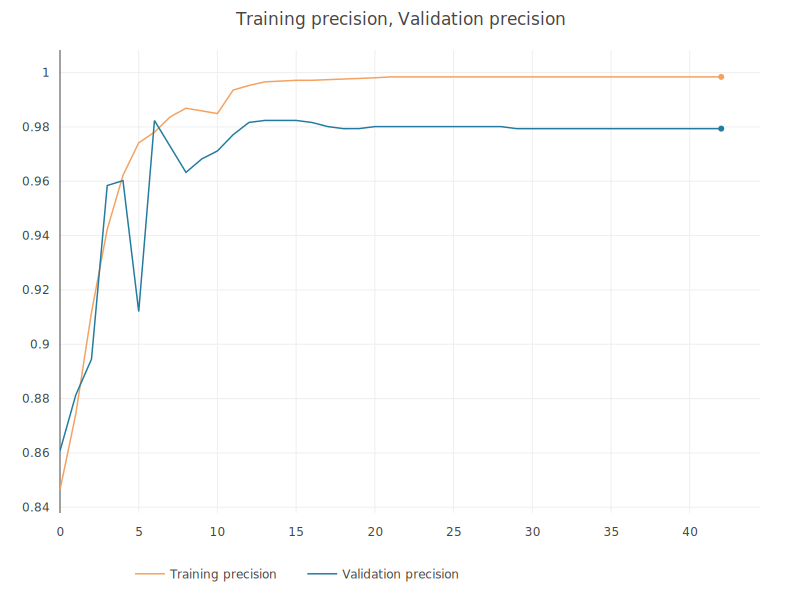
\includegraphics[height = 6cm]{Images/precision.pdf}
		\subcaption{CNN with FC layers at the end}
	\end{subfigure}
	\hspace{1mm}
	\begin{subfigure}{0.49\textwidth}
		\centering
		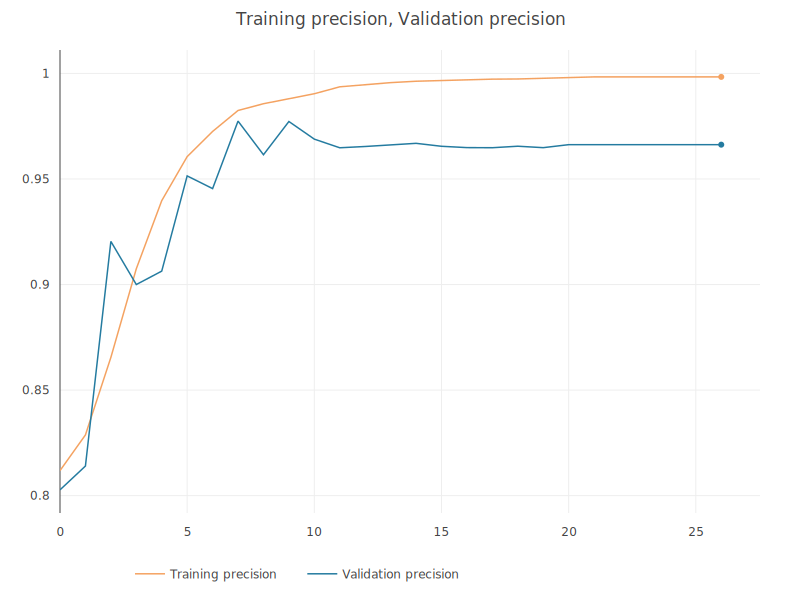
\includegraphics[height = 6cm]{Images/precision1.pdf}
		\subcaption{MDCNN}
	\end{subfigure}
	
	\caption{Training and validation precision at each epoch}
\end{figure*}

\begin{figure*}[h]
	\centering

	\begin{subfigure}{0.49\textwidth}
		\centering
		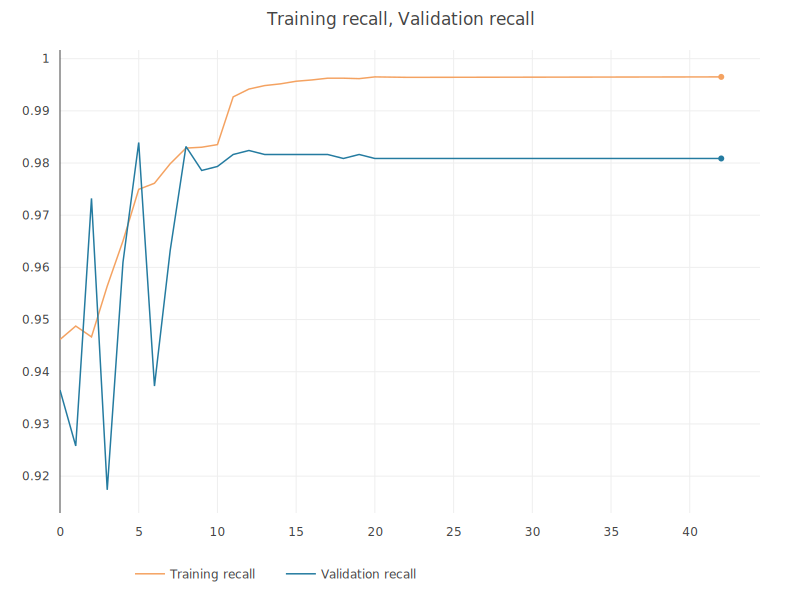
\includegraphics[height = 6cm]{Images/recall.pdf}
		\subcaption{CNN with FC layers at the end}
	\end{subfigure}
	\hspace{1mm}
	\begin{subfigure}{0.49\textwidth}
		\centering
		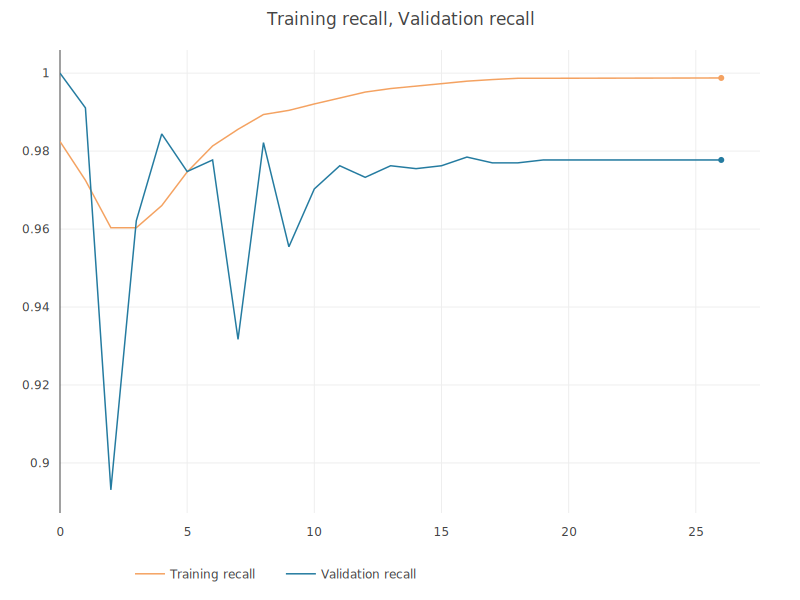
\includegraphics[height = 6cm]{Images/recall1.pdf}
		\subcaption{MDCNN}
	\end{subfigure}
	
	\caption{Training and validation recall at each epoch}
\end{figure*}

\begin{table}[H]
	\caption{Metrics on Multi-Dimensional Convolutional Networks (some test data is mixed with training data)}
	\centering
	\begin{tabular}{llll}
		\toprule
		Metric & Train set & Validation set & Test set
		\\
		\midrule
		Accuracy & 99.59 & 96.84 & 82.84
		\\
		Precision & 99.84 & 97.94 & 79.52
		\\
		Recall & 99.65 & 98.09 & 82.50
		\\
		F1 score & 99.75 & 98.01 & 80.98
		\\
		\bottomrule
	\end{tabular}
\end{table}


\begin{table}[H]
	\caption{Metrics on convolutional networks with fully connected layers at the end (some test data is mixed with training data)}
	\centering
	\begin{tabular}{llll}
		\toprule
		Metric & Train set & Validation set & Test set
		\\
		\midrule
		Accuracy & 99.93 & 96.78 & 64.37
		\\
		Precision & 99.81 & 97.60 & 38.43
		\\
		Recall & 99.52 & 97.98 & 87.33
		\\
		F1 score & 99.66 & 97.79 & 55.52
		\\
		\bottomrule
	\end{tabular}
\end{table}


\begin{table}[H]
	\caption{Metrics on convolutional networks with fully connected layers at the end (without leaking any test data into the training data)}
	\centering
	\begin{tabular}{llll}
		\toprule
		Metric & Train set & Validation set & Test set
		\\
		\midrule
		Accuracy & 99.51 & 96.84 & 46.20
		\\
		Precision & 99.80 & 97.94 & 38.67
		\\
		Recall & 99.69 & 98.09 & 16.99
		\\
		F1 score & 99.74 & 98.01 & 23.61
		\\
		\bottomrule
	\end{tabular}
\end{table}

\section*{Conclusion}
In this work we introduce a novel CNN architecture and use it for brain tumor detection. It has been demonstrated that our method achieves state-of-the-art performance on the same. Much work has been done to study what a CNN learns by visualizing their kernels. Similar research for such networks, particularly in the region of transformation from two-dimensional convolutions to one-dimensional convolutions will provide a greater understanding of what neural networks learn and will also provide a greater insight on how neural networks work.

\section*{Acknowledgment}
The authors would like to thank MICCAI for providing the training dataset and Dr. Prathosh AP for providing the test dataset. We also thank Dr. Prathosh AP, Chahat Chawla, Gantavya Bhatt and Hritik Bansal for helpful discussions about the implementation details.

\bibliographystyle{ieeetr}
\bibliography{references}

\appendices
\section{Code and neural network architectures}

The code and experiments are available \url{https://www.comet.ml/mayank31398/tumor}

\begin{table}[H]
	\caption{MDCNN}
	\centering
	\begin{tabular}{lllll}
		\toprule
		Operation & Kernel & Filters & Pooling/Stride & Activation
		\\ 
		\midrule
		2D Convolution & 7 * 7 * 1 & 2 & Maxpool(2) & SELU
		\\
		2D Convolution & 5 * 5 * 2 & 4 & Stride(2) & SELU
		\\
		2D Convolution & 5 * 5 * 4 & 8 & Stride(2) & SELU
		\\
		2D Convolution & 5 * 5 * 8 & 16 & Stride(2) & SELU
		\\
		2D Convolution & 5 * 5 * 16 & 32 & Maxpool(2) & SELU
		\\
		2D Convolution & 3 * 3 * 32 & 64 & Maxpool(2) & SELU
		\\
		\midrule
		Operation & Kernel & Filters & Pooling/Stride & Activation
		\\
		\midrule
		1D Convolution & 5 * 1 & 2 & Maxpool(2) & SELU
		\\
		1D Convolution & 3 * 2 & 4 & Maxpool(2) & SELU
		\\
		1D Convolution & 3 * 4 & 4 & Maxpool(2) & SELU
		\\
		1D Convolution & 3 * 4 & 2 & Maxpool(2) & SELU
		\\
		1D Convolution & 2 * 2 & 1 & Maxpool(2) & Sigmoidd
		\\
		\bottomrule
	\end{tabular}
\end{table}

\begin{table}[H]
	\caption{ConvNet with FC layers at the end}
	\label{tab:architecture}
	\centering
	\begin{tabular}{lllll}
		\toprule
		Operation & Kernel & Filters & Pooling & Activation
		\\ 
		\midrule
		2D Convolution & 9 * 9 * 1 & 2 & Maxpool(2) & SELU
		\\
		2D Convolution & 9 * 9 * 2 & 4 & Maxpool(2) & SELU
		\\
		2D Convolution & 7 * 7 * 4 & 8 & Maxpool(2) & SELU
		\\
		2D Convolution & 7 * 7 * 8 & 16 & Maxpool(2) & SELU
		\\
		2D Convolution & 5 * 5 * 16 & 32 && SELU
		\\
		2D Convolution & 3 * 3 * 32 & 64 && SELU
		\\
		\midrule
		Operation & Input & Output && Activation
		\\
		\midrule
		Fully connected & 576 & 128 && SELU
		\\
		Fully connected & 128 & 32 && SELU
		\\
		Fully connected & 32 & 8 && SELU
		\\
		Fully connected & 8 & 2 && SELU
		\\
		Fully connected & 2 & 1 && Sigmoid
		\\
		\bottomrule
	\end{tabular}
\end{table}

\end{document}
